% !TEX program = pdflatex
\documentclass[10pt,aspectratio=169]{beamer}

\usepackage[utf8]{inputenc}
\usepackage[T1]{fontenc}
\usepackage[english]{babel}
\usepackage{lmodern}
\usepackage{microtype}
\usepackage{amsmath,amssymb,bm,mathtools}
\usepackage{booktabs,array}
\usepackage{graphicx}

\usetheme[numbering=fraction,progressbar=frametitle]{metropolis}
\setbeamertemplate{frame numbering}[fraction]
\setbeamertemplate{navigation symbols}{}

\definecolor{CourseBlue}{HTML}{1A3C68}
\definecolor{CourseGreen}{HTML}{216E39}
\definecolor{CourseGold}{HTML}{B8860B}
\definecolor{CourseRed}{HTML}{9A2C2C}
\definecolor{SoftBlue}{HTML}{F2F6FA}
\definecolor{SoftGreen}{HTML}{F1F8F3}
\definecolor{SoftRed}{HTML}{FFF3F3}

\setbeamercolor{normal text}{fg=black,bg=white}
\setbeamercolor{structure}{fg=CourseBlue}
\setbeamercolor{title}{fg=CourseBlue}
\setbeamerfont{title}{size=\Large,series=\bfseries}
\setbeamercolor{frametitle}{bg=CourseBlue,fg=white}
\setbeamerfont{frametitle}{series=\bfseries,size=\large}
\setbeamertemplate{frametitle}{
  \nointerlineskip
  \begin{beamercolorbox}[wd=\paperwidth,ht=3.2ex,dp=1.4ex,leftskip=1em,rightskip=1em]{frametitle}
    \usebeamerfont{frametitle}\insertframetitle
  \end{beamercolorbox}
}
\setbeamercolor{block title}{bg=CourseBlue,fg=white}
\setbeamercolor{block body}{bg=SoftBlue,fg=black}
\setbeamercolor{block title example}{bg=CourseGreen,fg=white}
\setbeamercolor{block body example}{bg=SoftGreen,fg=black}
\setbeamercolor{block title alerted}{bg=CourseRed,fg=white}
\setbeamercolor{block body alerted}{bg=SoftRed,fg=black}
\setbeamertemplate{blocks}[rounded][shadow=false]

\newenvironment{modelbox}{\begin{beamercolorbox}[rounded=true,sep=0.7em,wd=\textwidth]{block body}
  \textbf{\color{CourseBlue}MODEL}\quad}{\end{beamercolorbox}}
\newenvironment{marketbox}{\begin{beamercolorbox}[rounded=true,sep=0.7em,wd=\textwidth]{block body example}
  \textbf{\color{CourseGreen}NO-ARBITRAGE}\quad}{\end{beamercolorbox}}
\newenvironment{simplificationbox}{\begin{beamercolorbox}[rounded=true,sep=0.7em,wd=\textwidth]{block body alerted}
  \textbf{\color{CourseRed}WATCH OUT}\quad}{\end{beamercolorbox}}
\newenvironment{pausebox}{\begin{beamercolorbox}[rounded=true,sep=0.8em,wd=\textwidth]{block body}
  \textbf{\color{CourseGold}YOUR TURN}\quad}{\end{beamercolorbox}}

\newcommand{\dd}{\,\mathrm d}
\newcommand{\E}{\mathbb E}
\newcommand{\Pp}{\mathbb P}
\newcommand{\Q}{\mathbb Q}
\newcommand{\R}{\mathbb R}
\newcommand{\cF}{\mathcal F}
\newcommand{\1}{\mathbf 1}
\newcommand{\Ncdf}{\Phi}

\AtBeginSection[]{
  \begin{frame}[plain]
    \vfill
    {\Large\bfseries\color{CourseBlue}\insertsectionhead\par}
    \medskip
    {\color{CourseBlue}\rule{0.92\textwidth}{0.8pt}}
    \vfill
  \end{frame}
}

\title{Vanilla Options in Practice}
\subtitle{Payoffs, Black--Scholes benchmarks, and static-arbitrage diagnostics}
\author{}
\date{Lecture 9}

\begin{document}

\begin{frame}[plain]
  \vfill
  {\LARGE\bfseries\color{CourseBlue}Vanilla Options in Practice\par}
  \medskip
  {\large Payoffs, Black--Scholes benchmarks, and static-arbitrage diagnostics\par}
  \medskip
  {\color{CourseGold}\rule{0.94\textwidth}{0.8pt}}
  \medskip
  {Lecture 9\par}
  \vfill
\end{frame}

\begin{frame}{One question drives the whole lecture}
\begin{block}{The question}
Lecture 8 gave model-free principles for comparing claims. How do those
principles discipline the prices of the options traders quote every day?
\end{block}
\begin{enumerate}
  \item Build calls, puts, and simple option positions from their payoffs.
  \item Recover put--call parity from replication, then use it to diagnose a
        mispriced quote.
  \item Read Black--Scholes as a pricing benchmark and a language for risk.
  \item Turn dominance, monotonicity, and convexity into quote checks.
  \item Construct the trade whenever a check fails.
\end{enumerate}
\end{frame}

% ============================================================
\section{Payoffs and Market Language}
% ============================================================

\begin{frame}{A vanilla option is a simple right exercised at one date}
At maturity \(T\), the underlying trades at \(S_T\) and the strike is \(K\).
\begin{columns}[T,onlytextwidth]
\column{0.48\textwidth}
\begin{block}{European call}
The right to \emph{buy} one share for \(K\):
\[
\boxed{(S_T-K)^+.}
\]
It is exercised only when \(S_T>K\).
\end{block}
\column{0.48\textwidth}
\begin{exampleblock}{European put}
The right to \emph{sell} one share for \(K\):
\[
\boxed{(K-S_T)^+.}
\]
It is exercised only when \(S_T<K\).
\end{exampleblock}
\end{columns}
\begin{marketbox}
``European'' fixes the exercise date; it does not describe where the option
trades or who may hold it.
\end{marketbox}
\end{frame}

\begin{frame}{Can you fill in the two payoff tables?}
\begin{pausebox}
Take \(K=100\). Fill in the call and put payoffs when \(S_T=80\), \(100\),
and \(130\). Which contract protects a fall in the stock price?
\end{pausebox}
\pause
\medskip
\begin{center}
\begin{tabular}{c|ccc}
\toprule
\(S_T\) & \(80\) & \(100\) & \(130\)\\
\midrule
Call \((S_T-100)^+\) & \(0\) & \(0\) & \(30\)\\
Put \((100-S_T)^+\) & \(20\) & \(0\) & \(0\)\\
\bottomrule
\end{tabular}
\end{center}
\begin{block}{Reading the table}
The call has upside exposure; the put is downside insurance.
\end{block}
\end{frame}

\begin{frame}{Going short flips every payoff}
\begin{columns}[T,onlytextwidth]
\column{0.48\textwidth}
\begin{block}{Long position}
Buying the call gives \((S_T-K)^+\). Buying the put gives \((K-S_T)^+\).
\end{block}
\column{0.48\textwidth}
\begin{alertblock}{Short position}
Selling the same contracts gives \(-(S_T-K)^+\) and \(-(K-S_T)^+\).
The premium is received today; the obligation is carried to \(T\).
\end{alertblock}
\end{columns}
\begin{marketbox}
For no-arbitrage arguments, write the \emph{net} payoff of the whole trade,
including every long and short leg.
\end{marketbox}
\end{frame}

\begin{frame}{Moneyness says whether immediate exercise has value}
At time \(t\), compare spot \(S_t\) with strike \(K\).
\begin{center}
\begin{tabular}{c|ccc}
\toprule
 & In the money & At the money & Out of the money\\
\midrule
Call & \(S_t>K\) & \(S_t\approx K\) & \(S_t<K\)\\
Put  & \(S_t<K\) & \(S_t\approx K\) & \(S_t>K\)\\
\bottomrule
\end{tabular}
\end{center}
\begin{block}{Important distinction}
Moneyness uses \(S_t\), but the European option payoff is determined by
\(S_T\). An OTM option today may finish ITM.
\end{block}
\end{frame}

\begin{frame}{Which option has the most time value?}
\begin{pausebox}
Two one-year calls have the same spot \(S_t=100\), volatility, and rate.
Their strikes are \(80\), \(100\), and \(130\). Which one is most likely
to consist mainly of time value rather than intrinsic value?
\end{pausebox}
\pause
\begin{exampleblock}{Answer}
The \(K=100\) call is at the money. Its intrinsic value is zero, so nearly
all of its price is time value: the value of possible future moves. Deep ITM
and deep OTM options typically have less time value.
\end{exampleblock}
\end{frame}

\begin{frame}{A straddle buys movement in either direction}
A long straddle is one call plus one put, both with strike \(K\):
\[
(S_T-K)^+ + (K-S_T)^+=\boxed{|S_T-K|}.
\]
\begin{columns}[T,onlytextwidth]
\column{0.48\textwidth}
\begin{block}{When \(S_T\) is near \(K\)}
Both options expire with little or no payoff.
\end{block}
\column{0.48\textwidth}
\begin{exampleblock}{When \(S_T\) moves far}
One option pays, and the payoff grows with the distance from \(K\).
\end{exampleblock}
\end{columns}
\begin{marketbox}
The payoff is convex: uncertainty has value to the holder of the straddle.
\end{marketbox}
\end{frame}

\begin{frame}{Stock plus put creates a floor; stock minus call creates a cap}
\begin{columns}[T,onlytextwidth]
\column{0.48\textwidth}
\begin{block}{Protective put}
\[
S_T+(K-S_T)^+=\max(S_T,K).
\]
The investor keeps upside but cannot finish below \(K\).
\end{block}
\column{0.48\textwidth}
\begin{exampleblock}{Covered call}
\[
S_T-(S_T-K)^+=\min(S_T,K).
\]
The investor gives up upside above \(K\) for the call premium.
\end{exampleblock}
\end{columns}
\end{frame}

% ============================================================
\section{Put--Call Parity}
% ============================================================

\begin{frame}{Two portfolios produce the same terminal wealth}
Assume no dividends and let \(D_t=e^{-r(T-t)}\). Compare:
\begin{columns}[T,onlytextwidth]
\column{0.48\textwidth}
\begin{block}{Portfolio A}
One call plus cash growing to \(K\):
\[
(S_T-K)^+ + K.
\]
\end{block}
\column{0.48\textwidth}
\begin{exampleblock}{Portfolio B}
One put plus one share:
\[
(K-S_T)^+ + S_T.
\]
\end{exampleblock}
\end{columns}
\begin{pausebox}
Check both portfolios for \(S_T\le K\) and for \(S_T>K\). What common
payoff do they deliver?
\end{pausebox}
\end{frame}

\begin{frame}{The common payoff is \(\max(S_T,K)\)}
\begin{center}
\begin{tabular}{c|cc}
\toprule
 & \(S_T\le K\) & \(S_T>K\)\\
\midrule
Call + cash & \(0+K=K\) & \((S_T-K)+K=S_T\)\\
Put + stock & \((K-S_T)+S_T=K\) & \(0+S_T=S_T\)\\
\bottomrule
\end{tabular}
\end{center}
\begin{marketbox}
The law of one price gives
\[
\boxed{C_t+K D_t=P_t+S_t,\qquad C_t-P_t=S_t-KD_t.}
\]
\end{marketbox}
\end{frame}

\begin{frame}{Put--call parity is a model-free identity}
\[
\boxed{C_t-P_t=S_t-Ke^{-r(T-t)}.}
\]
\begin{block}{What parity does not need}
No lognormal distribution, volatility estimate, or Black--Scholes formula.
Only the same underlying, the same strike, the same maturity, and a tradable
funding account.
\end{block}
\begin{simplificationbox}
With continuous dividend yield \(q\), replace \(S_t\) by
\(S_te^{-q(T-t)}\). The no-dividend formula then creates a false arbitrage
signal.
\end{simplificationbox}
\end{frame}

\begin{frame}{Can parity recover a put quote?}
\begin{pausebox}
Let \(S_t=100\), \(K=100\), \(T-t=1\), \(r=5\%\), and \(C_t=10.45\).
Use put--call parity to compute the put price.
\end{pausebox}
\pause
\[
K e^{-r(T-t)}=100e^{-0.05}\approx95.12,
\]
\[
P_t=C_t-S_t+K e^{-r(T-t)}
=10.45-100+95.12
\boxed{\approx5.57.}
\]
\begin{block}{Reading the result}
Once three of the four inputs are known, parity fixes the fourth.
\end{block}
\end{frame}

\begin{frame}{A parity violation tells us exactly what to trade}
Suppose the market quotes \(C_t=12\), \(P_t=5\), \(S_t=100\), and
\(K e^{-r\tau}=95.12\).
\[
\underbrace{C_t+K e^{-r\tau}}_{107.12}
>
\underbrace{P_t+S_t}_{105}.
\]
\begin{pausebox}
Which portfolio is expensive? Specify a trade that produces cash today and
zero net payoff at maturity.
\end{pausebox}
\pause
\begin{exampleblock}{Trade}
Sell the call and borrow \(95.12\); buy the put and the share. The initial
receipt is \(107.12-105=2.12\). The two sides have identical terminal payoff.
\end{exampleblock}
\end{frame}

% ============================================================
\section{Black--Scholes as a Benchmark}
% ============================================================

\begin{frame}{Black--Scholes adds a model to the no-arbitrage framework}
\begin{modelbox}
Under the pricing measure \(\Q\), assume constant \(r\), constant
volatility \(\sigma\), no dividends, and
\[
\frac{\dd S_t}{S_t}=r\dd t+\sigma\dd W_t^{\Q}.
\]
\end{modelbox}
\begin{block}{What the model contributes}
It specifies a distribution for \(S_T\), so it produces a numerical price.
No-arbitrage alone gives relations and bounds, but not generally a unique
price for every claim.
\end{block}
\end{frame}

\begin{frame}{The call formula separates stock value from strike cost}
Let \(\tau=T-t\). The Black--Scholes call is
\[
\boxed{C_t=S_t\Ncdf(d_1)-Ke^{-r\tau}\Ncdf(d_2),}
\]
where
\[
d_1=\frac{\log(S_t/K)+(r+\tfrac12\sigma^2)\tau}{\sigma\sqrt{\tau}},
\qquad
d_2=d_1-\sigma\sqrt{\tau}.
\]
\begin{block}{A useful interpretation}
\(\Ncdf(d_2)=\Q(S_T>K\mid\cF_t)\) in this model: the risk-neutral chance
that the call finishes in the money.
\end{block}
\end{frame}

\begin{frame}{Can you price an at-the-money one-year call?}
\begin{pausebox}
Use \(S_t=K=100\), \(r=5\%\), \(\sigma=20\%\), and \(\tau=1\). Compute
\(d_1\), \(d_2\), then use \(\Ncdf(0.35)\approx0.6368\) and
\(\Ncdf(0.15)\approx0.5596\).
\end{pausebox}
\pause
\[
d_1=0.35,\qquad d_2=0.15,
\]
\[
C_t=100(0.6368)-100e^{-0.05}(0.5596)
\boxed{\approx10.45.}
\]
\begin{marketbox}
The put price is then \(5.57\), either from its formula or from parity.
\end{marketbox}
\end{frame}

\begin{frame}{The Greeks turn a price into a local risk report}
\begin{center}
\begin{tabular}{c|l}
\toprule
Greek & What it measures\\
\midrule
Delta \(\Delta=\partial_SV\) & sensitivity to a small stock move\\
Gamma \(\Gamma=\partial_{SS}V\) & how rapidly Delta changes\\
Vega \(\partial_\sigma V\) & sensitivity to implied volatility\\
Theta \(\partial_tV\) & sensitivity to passage of time\\
Rho \(\partial_rV\) & sensitivity to the interest rate\\
\bottomrule
\end{tabular}
\end{center}
\begin{block}{For a Black--Scholes call}
\[
\Delta_{\mathrm{call}}=\Ncdf(d_1),
\qquad
\Gamma=\frac{\Ncdf'(d_1)}{S_t\sigma\sqrt{\tau}}.
\]
Delta is the first-order hedge ratio; Gamma is why that hedge must be rebalanced.
\end{block}
\end{frame}

\begin{frame}{What does a call Delta of \(0.64\) mean?}
\begin{pausebox}
An option has \(\Delta=0.64\). For a small \(\$1\) rise in the stock,
what is the first-order change in the option price? How would you hedge a
short position in 100 such calls?
\end{pausebox}
\pause
\begin{exampleblock}{First-order answer}
The option gains about \(\$0.64\) per contract. A short position in 100 calls
has Delta \(-64\), so buying about 64 shares makes the portfolio locally
Delta-neutral.
\end{exampleblock}
\begin{simplificationbox}
Delta-neutral is not risk-free: Gamma, volatility, and discrete rehedging
still matter.
\end{simplificationbox}
\end{frame}

\begin{frame}{Higher volatility raises the value of a long call and put}
\begin{block}{Why}
The payoffs \((S_T-K)^+\) and \((K-S_T)^+\) are convex in \(S_T\). Holding
the mean fixed, a wider distribution puts more probability in the tails,
where the holder benefits but cannot lose below zero at maturity.
\end{block}
\begin{marketbox}
For standard European options, Vega is positive. A higher implied volatility
therefore means a higher price, all else equal.
\end{marketbox}
\end{frame}

\begin{frame}{Implied volatility is the market price written in model units}
Given a European call quote \(C_t^{\mathrm{mkt}}(K,T)\), hold
\(S_t,K,\tau=T-t,r\) fixed and solve for the volatility:
\[
C^{\mathrm{BS}}\!\left(S_t,K,\tau,r,\sigma_{\mathrm{imp},t}(K,T)\right)
=C_t^{\mathrm{mkt}}(K,T).
\]
Black--Scholes Vega is positive: the price increases with \(\sigma\), so
there is at most one solution. In practice, find it numerically.
\begin{block}{Why traders quote volatility}
It makes options with different strikes and maturities easier to compare than
their dollar premiums alone.
\end{block}
\begin{simplificationbox}
Implied volatility is extracted from today's option price. It is neither
historical realized volatility nor a guaranteed forecast of future volatility.
\end{simplificationbox}
\end{frame}

\begin{frame}{Two variables: strike and maturity}
For one underlying at a \textbf{fixed observation date \(t\)}, the market
quotes a whole \textbf{implied volatility surface}:
\[
\boxed{(K,T)\longmapsto\sigma_{\mathrm{imp},t}(K,T),\qquad T>t.}
\]
\begin{columns}[T,onlytextwidth]
\column{0.48\textwidth}
\begin{block}{Vary strike \(K\), fix maturity \(T\)}
One slice gives the \textbf{smile or skew}: how implied volatility changes
across strikes for the same expiry.
\end{block}
\column{0.48\textwidth}
\begin{block}{Vary maturity \(T\), fix strike \(K\)}
Another slice gives a \textbf{term structure}: how implied volatility changes
across expiries for the same strike.
\end{block}
\end{columns}
Equivalently use time to maturity \(\tau=T-t\). The subscript \(t\) records
the observation date: the entire surface can change tomorrow.
\smallskip

\textbf{Black--Scholes benchmark:} a flat surface, with the same constant
\(\sigma\) for every strike \emph{and} maturity.
\end{frame}

\begin{frame}{Reading the surface: a smile is only one slice}
Illustrative annualized implied volatilities at today's spot \(S_t=100\):
\begin{center}
\begin{tabular}{lccc}
\toprule
Time to maturity & \(K=90\) & \(K=100\) & \(K=110\)\\
\midrule
3 months & \(28\%\) & \(22\%\) & \(20\%\)\\
1 year   & \(25\%\) & \(21\%\) & \(20\%\)\\
2 years  & \(24\%\) & \(22\%\) & \(21\%\)\\
\bottomrule
\end{tabular}
\end{center}
\begin{itemize}
\item Read a \textbf{row}: at 3 months, lower strikes have higher implied
      volatility (a downside skew).
\item Read a \textbf{column}: at \(K=100\), implied volatility is
      \(22\%,21\%,22\%\). The term structure need not be monotone.
\end{itemize}
\begin{block}{Specify both coordinates}
``The implied volatility is \(22\%\)'' is incomplete without a strike and
a maturity. A quoted \(22\%\) is annualized even for a 3-month option.
\end{block}
\end{frame}

\begin{frame}{A downside skew is expensive crash insurance}
For an equity index, low-strike puts are OTM yet often display higher implied
volatility than ATM options.
\begin{columns}[T,onlytextwidth]
\column{0.48\textwidth}
\begin{block}{Market observation}
Investors demand protection against severe market falls, raising low-strike
put prices.
\end{block}
\column{0.48\textwidth}
\begin{exampleblock}{Model reading}
Feeding those high prices into Black--Scholes yields a high
\(\sigma_{\mathrm{imp}}\): the volatility skew.
\end{exampleblock}
\end{columns}
\begin{marketbox}
The skew is not itself an arbitrage. It is evidence that constant-volatility
Black--Scholes is an imperfect market description.
\end{marketbox}
\end{frame}

\begin{frame}{Market evidence: the S\&P 500 downside skew}
\begin{columns}[c,onlytextwidth]
\column{0.75\textwidth}
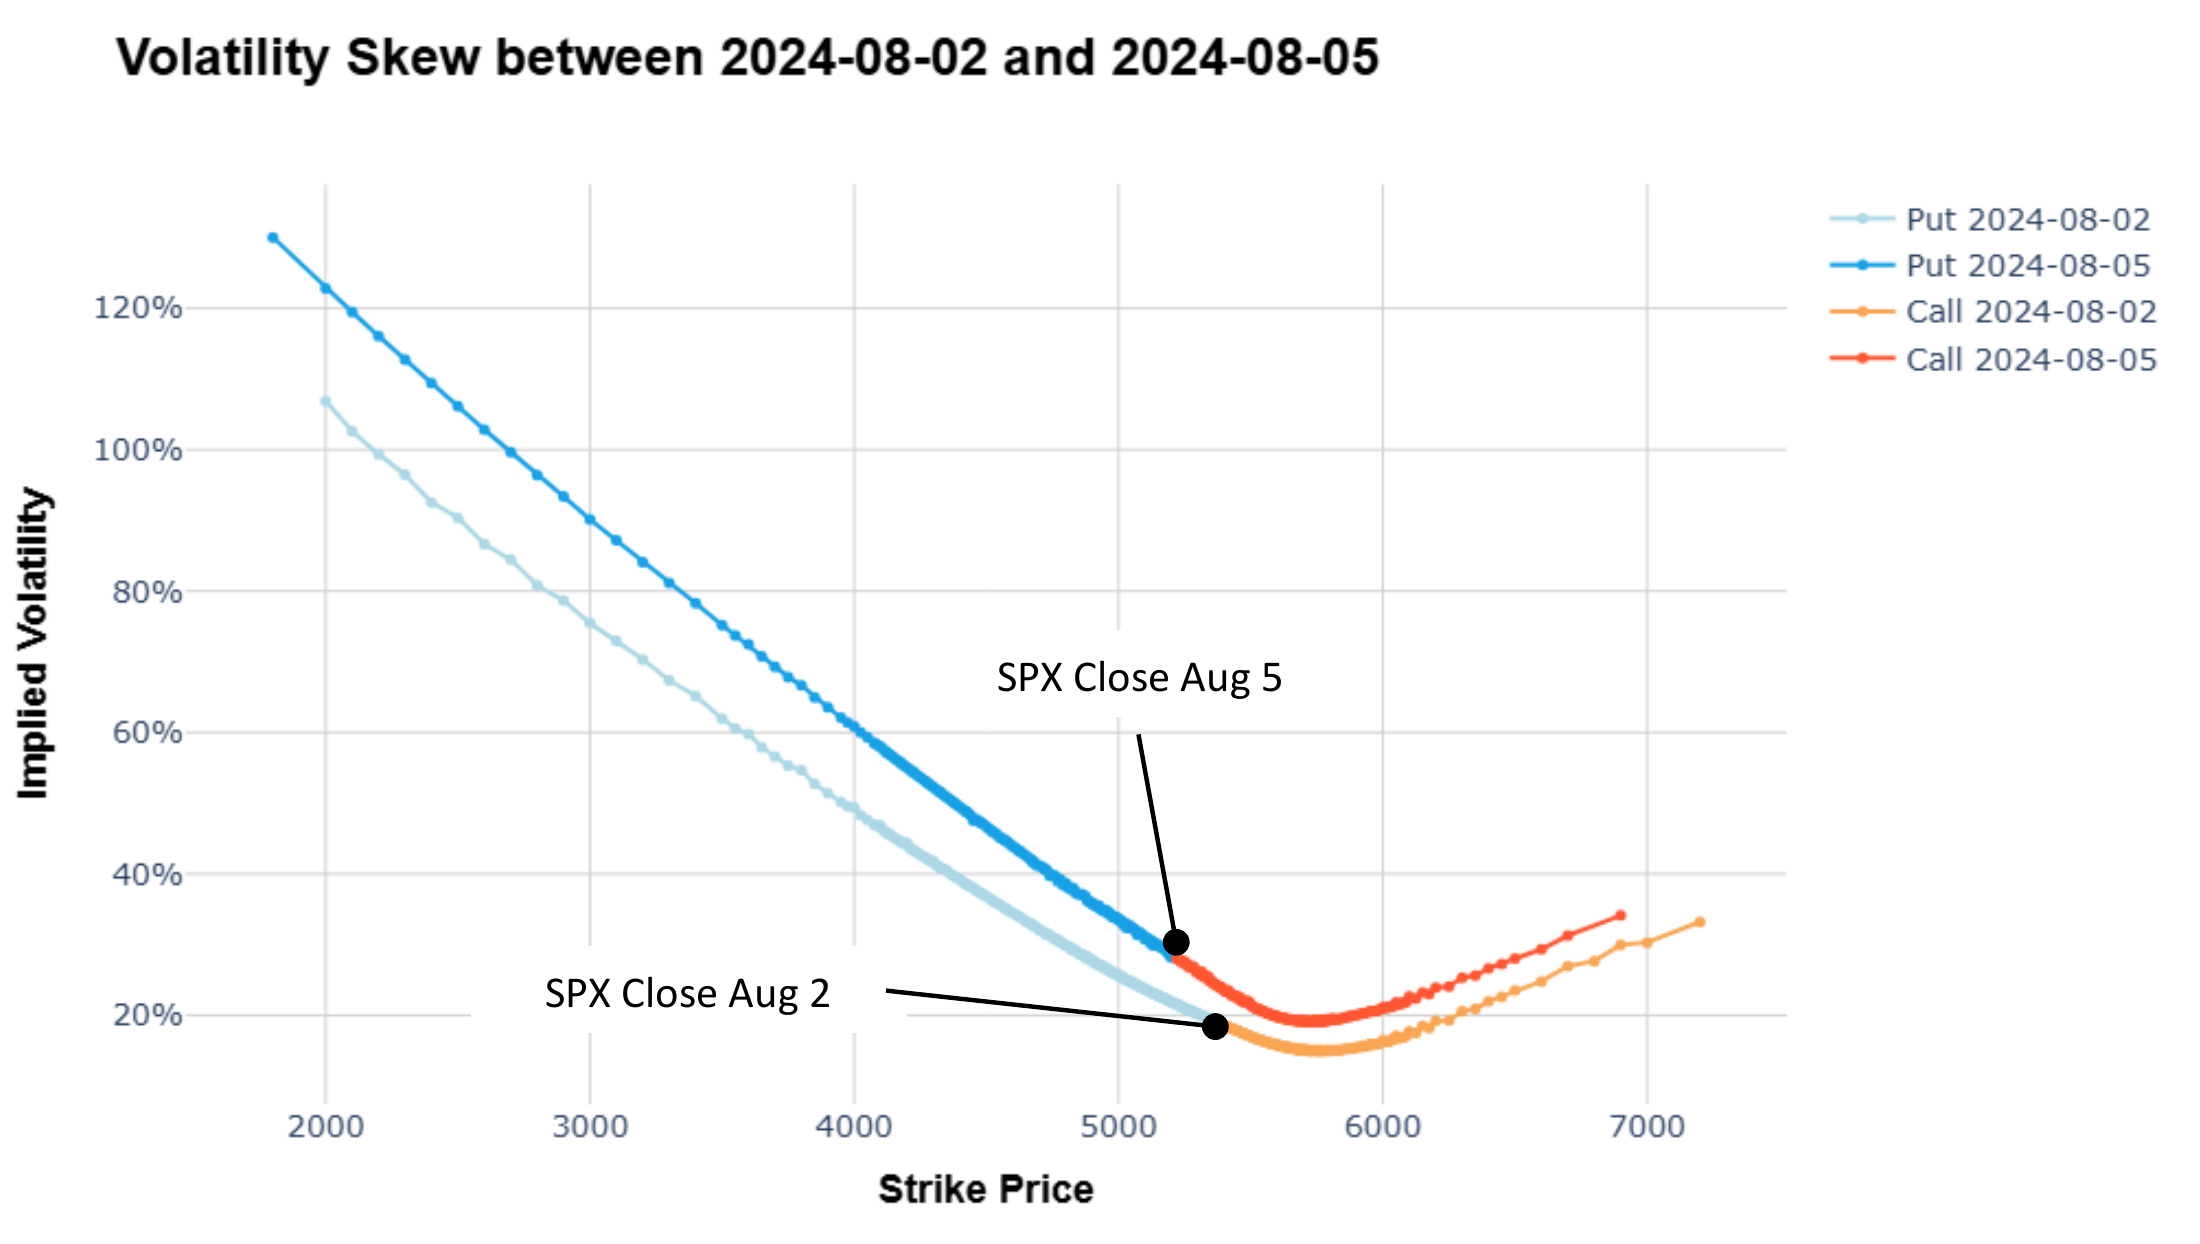
\includegraphics[width=\linewidth]{../Figures/spx_skew_2024-08-02_2024-08-05.png}
\column{0.23\textwidth}
\small
\textbf{30-day tenor}\\
2 and 5 August 2024.
\medskip

Around the money, lower strikes have higher implied volatilities.
\medskip

The curve also shifts between observation dates.
\end{columns}
\medskip
{\fontsize{6.5}{8}\selectfont
Source: \href{https://cdn.cboe.com/resources/vix/VIX-Decomposition-2025-08-01.pdf}{Cboe, \emph{The VIX Index Decomposition} (2025), Exhibit 7, p.~9}.
Market-based curves; 30-day tenor interpolated in variance between expiries.\par}
\end{frame}

\begin{frame}{Market evidence: a smile in EUR/USD options}
\begin{columns}[c,onlytextwidth]
\column{0.70\textwidth}
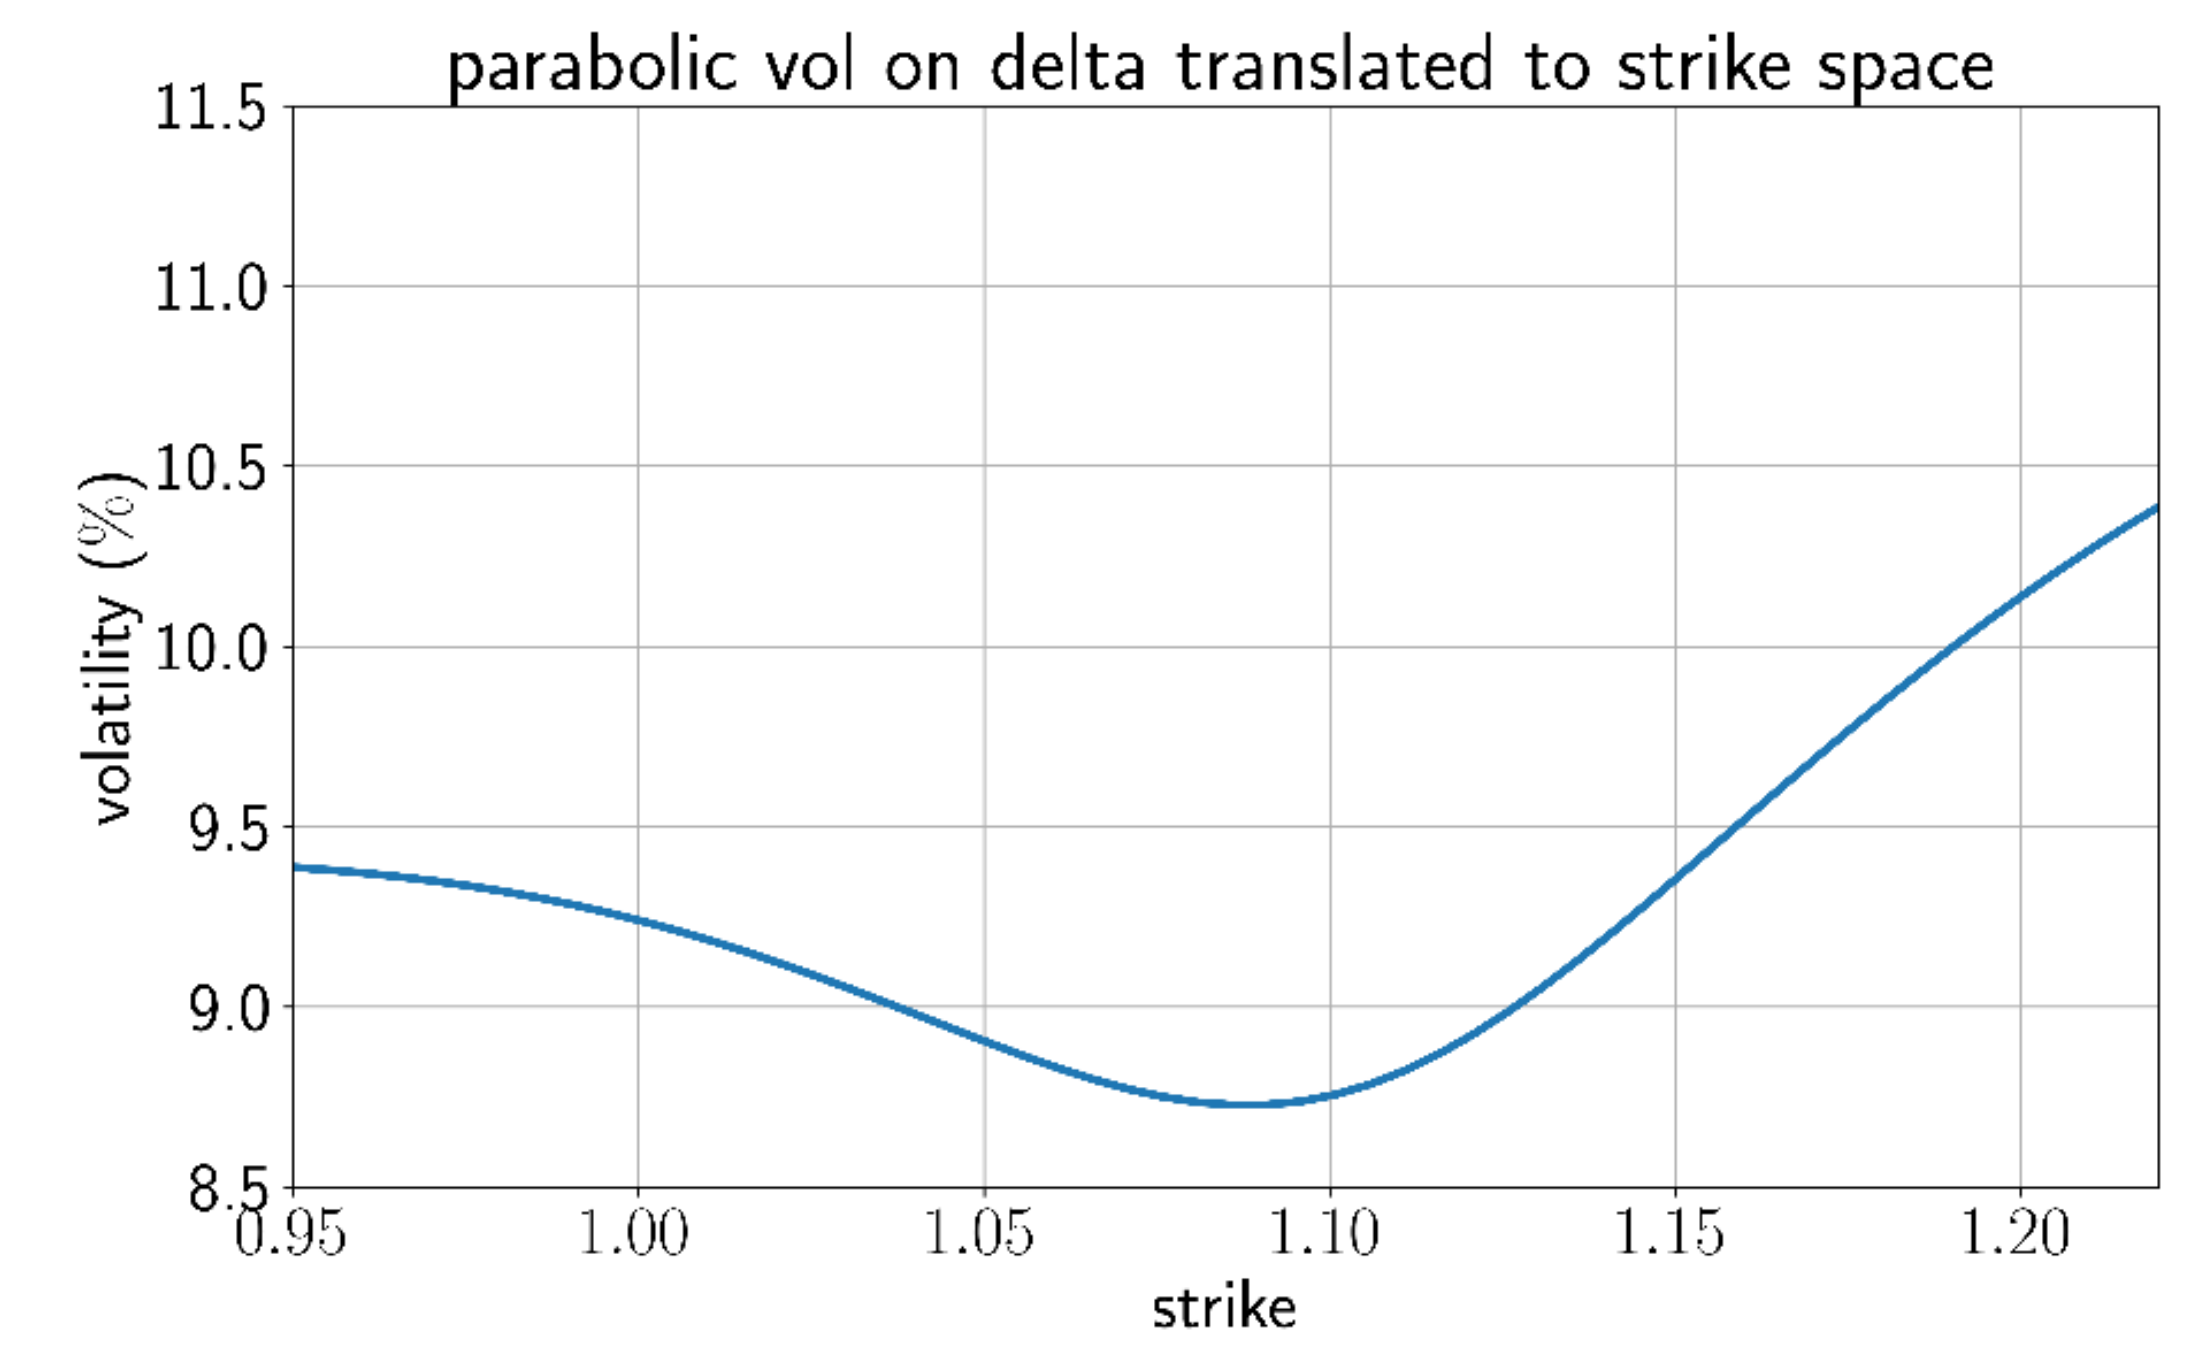
\includegraphics[width=\linewidth]{../Figures/eurusd_smile_2025-04-23.png}
\column{0.28\textwidth}
\small
\textbf{6-month tenor}\\
23 April 2025.
\medskip

Both wings rise above the trough: a \textbf{smile}.
\medskip

The smile need not be symmetric. Here the right wing is higher.
\medskip

\(K\): USD per EUR.
\end{columns}
\medskip
{\fontsize{6.5}{8}\selectfont
Source: \href{https://www.mathfinance.com/wp-content/uploads/2025/06/FX-Column_2025-07_Why-digitals-dont-have-percentage-prices.pdf}{U.~Wystup, MathFinance (2025), Figure 2}; ICE Data Services quotes.
Author's parabolic interpolation in delta, converted to strike; reference spot fixed at 1.1000.\par}
\end{frame}

% ============================================================
\section{Model-Free Bounds}
% ============================================================

\begin{frame}{No-arbitrage already pins an option price inside an interval}
Let \(D_t=e^{-r\tau}\), still assuming no dividends.
\begin{columns}[T,onlytextwidth]
\column{0.48\textwidth}
\begin{block}{Call}
\[
\boxed{\max(S_t-KD_t,0)\le C_t\le S_t.}
\]
\end{block}
\column{0.48\textwidth}
\begin{exampleblock}{Put}
\[
\boxed{\max(KD_t-S_t,0)\le P_t\le KD_t.}
\]
\end{exampleblock}
\end{columns}
\begin{marketbox}
These are model-free constraints. Black--Scholes prices must obey them, but
so must every arbitrage-free model.
\end{marketbox}
\end{frame}

\begin{frame}{The call upper bound comes from a superhedge}
One share always covers the call obligation:
\[
S_T\ge(S_T-K)^+.
\]
\begin{pausebox}
Suppose \(C_t>S_t\). What happens if you sell the call and buy the share?
Track the cashflow today and the payoff at \(T\).
\end{pausebox}
\pause
\begin{exampleblock}{Arbitrage}
Receive \(C_t-S_t>0\) today. At maturity, deliver the share if the call is
exercised; otherwise retain a share worth \(S_T\ge0\). The terminal net
payoff is nonnegative in every state.
\end{exampleblock}
\end{frame}

\begin{frame}{Parity plus positivity gives the call lower bound}
Put--call parity says
\[
C_t=P_t+S_t-KD_t.
\]
Since \(P_t\ge0\), \(C_t\ge S_t-KD_t\). Since a call payoff is nonnegative,
\(C_t\ge0\) as well. Together:
\[
\boxed{C_t\ge\max(S_t-KD_t,0).}
\]
\begin{block}{Same architecture as Lecture 8}
Use a payoff inequality first; then translate it into a price inequality.
\end{block}
\end{frame}

\begin{frame}{Are these quotes inside the arbitrage-free interval?}
\begin{pausebox}
Let \(S_t=100\), \(K=100\), \(r=5\%\), \(\tau=1\). Check call quotes
\(2\), \(10.45\), and \(103\) against the model-free bounds.
\end{pausebox}
\pause
\[
\max(100-100e^{-0.05},0)\approx4.88,
\qquad C_t\le100.
\]
\begin{center}
\begin{tabular}{c|ccc}
\toprule
Quote & \(2\) & \(10.45\) & \(103\)\\
\midrule
Verdict & too low & feasible & too high\\
\bottomrule
\end{tabular}
\end{center}
\end{frame}

\begin{frame}{Superhedges and subhedges generalize the same logic}
If a liquid strategy satisfies \(Y_T\le H\le X_T\), then its initial costs
give the interval
\[
\boxed{Y_0\le \text{price}(H)\le X_0.}
\]
\begin{columns}[T,onlytextwidth]
\column{0.48\textwidth}
\begin{block}{Claim too expensive}
Sell \(H\), buy the superhedge \(X\), and keep the difference.
\end{block}
\column{0.48\textwidth}
\begin{exampleblock}{Claim too cheap}
Buy \(H\), short the subhedge \(Y\), and keep the difference.
\end{exampleblock}
\end{columns}
\end{frame}

% ============================================================
\section{The Shape of an Arbitrage-Free Option Surface}
% ============================================================

\begin{frame}{A higher strike can never make the same call more valuable}
For \(K_1<K_2\),
\[
(S_T-K_1)^+\ge(S_T-K_2)^+
\qquad\text{in every state.}
\]
The dominance principle gives
\[
\boxed{C_t(K_1)\ge C_t(K_2).}
\]
\begin{block}{For puts, the direction reverses}
\[
P_t(K_1)\le P_t(K_2).
\]
The right to sell at a higher price is more valuable.
\end{block}
\end{frame}

\begin{frame}{Can you exploit a monotonicity violation?}
\begin{pausebox}
Two calls share the same maturity and have \(K_1=90<K_2=110\), but the
market quotes \(C_t(90)=8\) and \(C_t(110)=10\). State the trade and explain
why it cannot lose at maturity.
\end{pausebox}
\pause
\begin{exampleblock}{Trade}
Buy the lower-strike call for \(8\), sell the higher-strike call for \(10\),
and receive \(2\) today. The terminal payoff
\[
(S_T-90)^+-(S_T-110)^+\ge0
\]
in every state.
\end{exampleblock}
\end{frame}

\begin{frame}{Convexity says call prices cannot bend the wrong way}
For equally spaced strikes \(K-h<K<K+h\), the butterfly payoff is
\[
(S_T-K+h)^+-2(S_T-K)^++(S_T-K-h)^+\ge0.
\]
Therefore its price must be nonnegative:
\[
\boxed{C_t(K-h)-2C_t(K)+C_t(K+h)\ge0.}
\]
\begin{marketbox}
Equivalently, \(K\mapsto C_t(K)\) is decreasing and convex. These are
requirements on the entire strip of option quotes, not on one option alone.
\end{marketbox}
\end{frame}

\begin{frame}{Why is the butterfly payoff never negative?}
\begin{pausebox}
Let the strikes be \(90\), \(100\), and \(110\). Evaluate the butterfly
payoff for \(S_T\le90\), \(90<S_T<100\), \(100\le S_T<110\), and
\(S_T\ge110\).
\end{pausebox}
\pause
\begin{center}
\begin{tabular}{c|c}
\toprule
Region & payoff\\
\midrule
\(S_T\le90\) & \(0\)\\
\(90<S_T<100\) & \(S_T-90\)\\
\(100\le S_T<110\) & \(110-S_T\)\\
\(S_T\ge110\) & \(0\)\\
\bottomrule
\end{tabular}
\end{center}
It is a nonnegative tent, peaking at \(10\) when \(S_T=100\).
\end{frame}

\begin{frame}{A three-quote diagnostic finds a butterfly arbitrage}
Same maturity and underlying; the market quotes
\[
C_t(90)=14,\qquad C_t(100)=12,\qquad C_t(110)=7.
\]
\begin{pausebox}
Check monotonicity first, then convexity. If a condition fails, name the
portfolio and compute its initial cashflow.
\end{pausebox}
\pause
\begin{block}{Monotonicity}
\(14>12>7\): no problem.
\end{block}
\begin{alertblock}{Convexity}
Convexity needs \(C_t(100)\le\tfrac12(14+7)=10.5\), but \(12>10.5\).
The middle strike is overpriced relative to the wings.
\end{alertblock}
\end{frame}

\begin{frame}{Selling the expensive middle strike creates the arbitrage}
Buy \(C_t(90)\) and \(C_t(110)\); sell two \(C_t(100)\):
\[
\text{initial cost}=14+7-2(12)=\boxed{-3}.
\]
The trader receives \(3\) today and holds the nonnegative butterfly payoff
at maturity.
\begin{marketbox}
\[
\text{payoff shape}\ \longrightarrow\ \text{price inequality}\ \longrightarrow\ \text{explicit trade}.
\]
\end{marketbox}
\end{frame}

\begin{frame}{More time is valuable under a clean comparison}
For a fixed strike, suppose \(T_1<T_2\), rates and dividends are zero.
Then
\[
\boxed{C_t(K,T_2)\ge C_t(K,T_1).}
\]
\begin{block}{Calendar-spread logic}
If the longer call were cheaper, buy it and sell the shorter call. The trade
generates cash today. At \(T_1\), the remaining longer option is worth at
least the intrinsic value needed to settle the short option.
\end{block}
\begin{simplificationbox}
With rates or dividends, maturity comparisons require more care. Do not use
this simple monotonicity statement without its assumptions.
\end{simplificationbox}
\end{frame}

% ============================================================
\section{Synthesis: Diagnose Before You Price}
% ============================================================

\begin{frame}{A disciplined order for checking an option quote}
\begin{enumerate}
  \item Identify the exact contract: underlying, strike, maturity, dividends.
  \item Check positivity and the basic upper and lower bounds.
  \item Pair calls and puts with the same \(K,T\) to check parity.
  \item Across strikes, check monotonicity and convexity.
  \item Across maturities, apply calendar checks only with the right assumptions.
  \item If a check fails, write the portfolio before calling it an arbitrage.
\end{enumerate}
\begin{marketbox}
Black--Scholes provides a benchmark and an implied volatility; it never
replaces model-free consistency checks.
\end{marketbox}
\end{frame}

\begin{frame}{Final challenge: build the trade, not just the inequality}
Same maturity and stock; assume no dividends. The quotes are
\[
S_t=100,\quad K=100,\quad r=5\%,\quad \tau=1,
\quad C_t=12,\quad P_t=5.
\]
\begin{pausebox}
Is put--call parity satisfied? If not, write each leg of a zero-terminal-payoff
arbitrage and its initial receipt.
\end{pausebox}
\pause
\[
C_t+100e^{-0.05}=107.12>105=P_t+S_t.
\]
Sell the call, borrow \(95.12\), buy the put, and buy one share. The receipt
is \(2.12\) today; parity makes the terminal net payoff zero.
\end{frame}

\begin{frame}{The big picture in one line}
\[
\boxed{\text{option payoff geometry}
\quad\Longrightarrow\quad
\text{arbitrage-free prices and hedges}.}
\]
\begin{block}{What to retain}
Calls and puts are simple contingent claims. Replication gives parity;
dominance gives bounds; strike convexity gives butterfly tests. Black--Scholes
turns the same contracts into prices, Greeks, and implied volatilities.
\end{block}
\begin{marketbox}
The habit to keep: every price statement should be backed by a payoff
comparison or an explicit trading strategy.
\end{marketbox}
\end{frame}

\end{document}
